\chapter{Implementation in the \tnreason package}\label{cha:implementation}

We here document the implementation of the discussed concepts in the \python package \tnreason, in the version \curvertnreason
 
 % Name
\tnreason is an abbreviation of \textbf{t}ensor \textbf{n}etwork \textbf{reason}ing, by which we emphasize the capabilities of this package to represent and answer reasoning tasks by tensor network contractions. 

% Installation
The package can be installed either by cloning the repository
\begin{center}
	\href{https://github.com/EnexaProject/enexa-tensor-reasoning}{https://github.com/EnexaProject/enexa-tensor-reasoning}
\end{center}
or by
\begin{lstlisting}
	!pip install tnreason==2.0.0
\end{lstlisting}

\sect{Architecture}

\tnreason is structured in four subpackages and three layers
\begin{itemize}
	\item Layer 1: Storage and numerical manipulations, by subpackage \spengine, "Tensor Networks" -> building "tn" of \tnreason
	\item Layer 2: Specification of workload, subpackage \sprepresentation specific for storage, subpackage \spreasoning specific for manipulations
	\item Layer 3: Applications in reasoning, by subpackage \spapplication, "Reasoning" -> building "reason" of \tnreason
\end{itemize}

We sketch this structure by
\begin{center}
\input{./OtherContent/tikz_pics/implementation/architecture_sketch.tex}
\end{center}


\sect{Implementation of basic notation}

First of all, we explain how the basis notation explained in \charef{cha:notation} is reflected in the implementation.

\subsect{\bncategoricals}
Categorical Variables are identified by strings, which then appear as colors of the corresponding tensor axes.
Their dimension is stored in shapeDicts, but most practically these shapes are stored in the tensors in which variables appear.
Suffixes in the color string (defined in \inlinecode{representation.suffixes}) denote the type of the variable:
\begin{itemize}
	\item Distributed variables with color suffix \disVarSuf: $\catvariableof{\cdot}$
	\item Computed variables with color suffix \comVarSuf: $\headvariableof{\cdot}$
	\item Selection variables with color suffix \selVarSuf: $\selvariableof{\cdot}$
	\item Term variables with color suffix \terVarSuf: $\indvariableof{\cdot}$
\end{itemize}

\subsect{\bntensors}
\paragraph{Tensors} are objects of classes inheriting \inlinecode{engine.TensorCore} with main attributes
\begin{itemize}
	\item \inlinecode{values}: Storing the coordinates of the tensors (individual realization for different cores)
	\item \inlinecode{colors}: List of the variables $[\headvariableof{\formula},\catvariableof{0},\catvariableof{1}]$
	\item \inlinecode{name}: Reflecting the notation such as $\rencodingof{\formula}$
	\item \inlinecode{shape}: Storing the dimension of each appearing variable, as a list of integers with the same length as colors.
\end{itemize}

Suffixes in the name string (defined in \inlinecode{representation.suffixes}) highlight the origin and purpose of the tensor.
Cores are named with suffixes based on their functionality
\begin{itemize}
	\item Computation core with name suffix \comCoreSuf: They represent the computation of a function in basis calculus, and are directed cores.
		Their colors are \inlinecode{[headColors] + [inputColors]}, where \inlinecode{[inputColors]} are either distributed variables or, if having a composition of formulas.
		When the function is a selection augmentation of other functions, selection colors are listed in the end of \inlinecode{[inputColors]}.
	\item Activation core with name suffix \actCoreSuf: two-dimensional vectors representing of the activation core to a formula
\end{itemize}

Exploiting efficient representation tricks we further have the tensor name suffices:
\begin{itemize}
	\item \atoCoreSuf: Atomization core, for sparse representation of categorical constraints
	\item \vselCoreSuf: Variable selection core: For sparse representation of variable selectors
\end{itemize}

Tensors are instantiated by
\begin{lstlisting}
	engine.getCore(coreType)(values, colors, name, shape)
\end{lstlisting}
where \inlinecode{coreType} is a string further specifying a specific implementation of tensors (see for more detail \secref{sec:implementationEngine}).
The default tensor implementation \defaultCoreType is chosen, when \inlinecode{coreType} is not specified.



One-hot encodings are specific tensors created in \sprepresentation.

\subsect{\bncontractions}
\paragraph{Tensor networks} are stored as dictionaries of tensors, where the keys coincide with the names of the corresponding tensors.

\paragraph{Contractions} are implemented in the subpackage \spengine, orienting on \defref{def:contraction}.
Reflected in the notation
\begin{align*}
	\contractionof{\tnetof{\graph}}{\secnodevariables}
\end{align*}
a contraction is defined by
\begin{itemize}
	\item Tensor Network $\tnetof{\graph}$, specified by a dictionary of tensor names as keys and valued by tensor cores.
	\item Open Variables $\secnodes$, specified by a list of colors to the variables.
\end{itemize}
Contraction calls are implemented as
\begin{lstlisting}
	engine.contract(contractionMethod, coreDict, openColors, dimensionDict, evidenceColorDict)
\end{lstlisting}
where the arguments are
\begin{itemize}
	\item \inlinecode{contractionMethod}: str, chooses one of the contraction providers. The default contraction method \defaultContractionMethod is chosen, when
	\item \inlinecode{coreDict}: Dictionary of TensorCores (of the above formats), representing the Tensor Network $\tnetof{\graph}$
	\item \inlinecode{openColors}: List of str, each str identifying a color, that is a variable to be left open in the contraction
	\item \inlinecode{dimensionDict}: Dict valued by int and keys by str, storing dimensions to each variable. This is of optional usage, when a color in openColors does not appear in the coreDict.
	\item \inlinecode{evidenceColorDict}: Dict valued by int and keys by str, indicating sliced variables
\end{itemize}

Coordinates of tensors can be retrieved by
\begin{align*}
	\contractionof{\hypercoreat{\nodevariables}}{\secnodevariables=\catindexof{\secnodes}} \, .
\end{align*}
We implement this by leaving \inlinecode{openColors} empty and passing $\catindexof{\secnodes}$ as the \inlinecode{evidenceColorDict}, as a dictionary with keys by the \inlinecode{str} colors to the variables and values by the corresponding \inlinecode{int} indices.

Graphical illustrations can be generated by
\begin{lstlisting}
	engine.draw_factor_graph(coreDict)
\end{lstlisting}
where \inlinecode{coreDict} is a tensor network to be visualized.


\subsect{\bnencoding}
Encoding schemes are implemented in the subpackage \sprepresentation.



\sect{Subpackage \spengine}\label{sec:implementationEngine}

The \spengine subpackage is for the storage and numerical manipulation of tensors and tensor networks.
We organize the subpackage as the lowest layer of \tnreason, specializing in storage of Tensor Networks and performing the contractions.

\subsect{Cores}

\paragraph{Iterator based Core Initialization}
We orient on basis+ sparse tensor decomposition in the initialization of tensor cores, as discussed in detail in \charef{cha:sparseCalculus}.
An elementary basis+ tensor is specified by tuples
\begin{lstlisting}
	(value, posDict)
\end{lstlisting}
where \inlinecode{posDict} specifies the values to the variables, which do not have a trivial leg vector, and \inlinecode{value} a scalar scaling the basis vector.
Comparing with the notation of \charef{cha:sparseCalculus}, the keys of \inlinecode{posDict} correspond with $\variableset$, the values of \inlinecode{posDict} with $\catindexof{\variableset}$ and \inlinecode{value} corresponds with $\slicescalar$.

A basis+ $\cpformat$ tensor is specified by an iterator \inlinecode{sliceIterator} over elementary basis+ tensors, where the $\cpformat$ rank is the length of the iterator
Given such a representation a tensor is instantiated by
\begin{lstlisting}
	engine.create_from_slice_iterator(shape, colors, sliceIterator, coreType, name)
\end{lstlisting}
where \inlinecode{shape, colors, coreType, name} are used in the call of an empty core by \inlinecode{engine.get_core} and \inlinecode{sliceIterator} used to iterative add the basis+ elementary tensors to create the tensor.

\paragraph{Core Arithmetics}
When executing
\begin{lstlisting}
	exampleCore[posDict] = value
\end{lstlisting}
we add a basis+ tensor specified by \inlinecode{posDict}, that is
\begin{align*}
	\hypercoreat{\shortcatvariables} \algdefsymbol \hypercoreat{\shortcatvariables} + \contractionof{\onehotmapofat{\catindexof{\variableset}}{\catvariableof{\variableset}}}{\shortcatvariables} \, .
\end{align*}
The linear structure of tensors spaces are reflected in sums of tensors implemented with the same \inlinecode{coreType}, as
\begin{lstlisting}
	summed = exampleCore1 + exampleCore2
\end{lstlisting}
and scalar multiplication, where a scalar \inlinecode{value} of type \inlinecode{int} or \inlinecode{float}
\begin{lstlisting}
	multiplied = value * exampleCore
\end{lstlisting}
Both operations are performed as manipulations of the tensors \inlinecode{values}.
Contraction of two cores
\begin{lstlisting}
	contracted = exampleCore1.contract_with(exampleCore2)
\end{lstlisting}
these are especially used in corewise contraction, where \inlinecode{contractionMethod="CoreWiseContractor"}.


\subsect{Contractions}

\textbf{Cores}

%Each Tensor core has attributes
%\begin{itemize}
%	\item values (array-like): storing the value of the coordinates
%	\item colors (list of str): specifying the name of the variables represented by its axes
%	\item name (str): to distinguish from other cores
%\end{itemize}
%The implemented core types differ in the values argument.


\textbf{Polynomial Cores}
Polynomial Cores are implementations of the monomial decomposition or basis+ (see \defref{def:polynomialSparsity}).
Here the each tuple $(\lambda,\variableset,\catvariableof{\variableset})$ is stored as a tuple of the scalar $\lambda$ and a dictionary with $\variableset$ as keys and $\catvariableof{\variableset}$ as values.

\red{The spare cores (Polynomial and Pandas Core) exploit the matrix representation of \remref{rem:matSotrageBasPlus}.}

% Contraction Method List
The supported cores are
\begin{center}
\begin{tabular}{|c|c|c|}
  	\hline
 	\textbf{coreType} & \textbf{Package} & \text{Explanation}  \\
  	\hline
 	\stringof{NumpyTensorCore} 	&  $\mathrm{numpy}$  & Numpy array storing the values\\
  	\hline
 	\stringof{PolynomialCore} 	&  $\mathrm{numpy}$  & Storing the values in a basis+ $\cpformat$ Decomposition\\
  	\hline
\end{tabular}
\end{center}


\textbf{Binary CP Decomposition}

Based on the monomial decomposition $\slicesparsityof{\cdot}$ as specified in \defref{def:polynomialSparsity}.
To store the values of a tensor we store the slices of tensors by the indices $\catindexof{\variableset}$. 

% Trick -> To BinaryCP
Contractions can be performed by partially contracting the cores of the decomposition.
In this way, one can avoids coordinatewise storages of high-order tensors, which can be intractable.

\textbf{Tensor Networks}

Tensor networks $\tnetof{\graph}$ are defined by hypergraphs with hyperedges decorated by tensor cores. 
We store them by dictionaries with values being tensor cores and keys coinciding with the name of each tensor core.


% Contraction Method List
The supported contraction methods are
\begin{center}
\begin{tabular}{|c|c|c|}
  	\hline
 	\textbf{contractionMethod} (str) & \textbf{Package} & \text{Explanation}  \\
  	\hline
 	\stringof{NumpyEinsum} 	&  $\mathrm{numpy}$  & Einstein summation of $\mathrm{numpy}$ arrays\\
  	\hline
 	\stringof{TensorFlowEinsum} 	&  $\mathrm{tensorflow}$  & Einstein summation of $\mathrm{tensorflow}$ tensors\\
  	\hline
	\stringof{TorchEinsum} 	&  $\mathrm{torch}$  & Einstein summation of $\mathrm{torch}$ tensors\\
  	\hline
	\stringof{TentrisEinsum} 	&  $\mathrm{tentris}$  & Einstein summation of $\mathrm{tentris}$ hypertries\\
  	\hline
	\stringof{PgmpyVariableEliminator} 	&  $\mathrm{pgmpy}$  & Variable Elimination of DiscreteFactors in $\mathrm{pgmpy}$\\
  	\hline
	\stringof{CorewiseContractor} 	&  $\mathrm{numpy}$  & Contraction of CP Decompositions stored in $\mathrm{numpy}$ arrays\\
  	\hline	
\end{tabular}
\end{center}


%%\textbf{Einstein Summation}
%Contractions represented as Einstein summation, as implemented in:
%\begin{itemize}
%	\item numpy
%	\item tensorflow
%	\item pytorch
%	\item tentris
%\end{itemize}

%\textbf{Variable Elimination}
%Contractions can be executed by variable elimination as implemented in:
%\begin{itemize}
%	\item pgmpy
%\end{itemize}

%\textbf{Manipulation of Binary CP Decomposition}
%Contraction of tensors in Binary CP Decomposition as in \secref{sec:BinaryCPManipulation}.







\sect{Subpackage \sprepresentation}\label{sec:implementationRepresentation}

The \sprepresentation subpackage consists in a collection of core creation methods.

Here the relational encodings $\rencodingof{\exfunction}$ of various maps $\exfunction$ are created.


We arrange the \sprepresentation subpackage into the second layer of the \tnreason architecture, since it specifies tensor cores which formats are specified in \spengine.




\textbf{Coordinate Calculus}

Main function
\begin{lstlisting}
	engine.coordinatewise_transform(coresList, transformFunction)
\end{lstlisting}

\textbf{Basis Calculus}

Main function
\begin{lstlisting}
	engine.relational_encoding()
\end{lstlisting}
basis calculus then based on contractions.







\subsect{Refinement by infixes}

Both the cores and the colors are further refined by infixes before the suffices to denote specific instantiations.

\begin{itemize}
	\item \selCoreIn: Involving a selection variable
	\item \eviCoreIn: Storing evidence about a variable
	\item \heaIn: Head of a function, typically the variable computed at a activation selector
	\item \funIn: Function selection variables
	\item \posIn+\stringof{i}: Variable selection for argument at position $i$
	\item \datIn: Involving data (data cores and colors)
\end{itemize}

Further infixes are strings denoting atom names and neuron neames.


\subsect{Relational encoding of formulas} % -> To application!

Propositional formulas $\exformula$ are represented in three schemes:
\begin{itemize}
	\item Script language $\synencodingof{\exformula}$ by nested lists (see \secref{subsec:scriptLanguage}).
		Most practical to choose a formula from a neuro-symbolic architecture.
	\item Strings specifying the categorical variables $\catvariableof{\exformula}$.
	\item Representation of formulas by tensor networks being contracted to $\rencodingof{\exformula}$
\end{itemize}

Conversions of the formats:
\begin{itemize}
	\item $\synencodingof{\exformula}$ to color by
		\begin{lstlisting}
			representation.get_formula_color($\synencodingof{\exformula}$)
		\end{lstlisting}
		Here the nested lists are turned in a string by concatenating all elements of a list with \stringof{\_} and adding \stringof{[} and \stringof{]} at the beginning and end of each list.
	\item  $\synencodingof{\exformula}$ to tensor network
		\begin{lstlisting}
			representation.create_raw_cores($\synencodingof{\exformula}$)
		\end{lstlisting}
		This creates the connective cores for the semantic representation of $\rencodingof{\exformula}$.
We encode them by
\end{itemize}

When encoding formulas with hard interpretation, we furthermore add a head core of type \stringof{truthEvaluation} since we have
 	\[ {\exformula} = \sbcontractionof{\rencodingof{\exformula},\tbasis}{\catvariableof{\exformula}} \, . \]



\subsect{Representation of MLNs}

\textbf{Computation Cores} are binary cores relating the variables in a predefined way, which is not changing during reasoning.
\begin{itemize}
	\item Logical interpretation: Cores $\rencodingof{\exconnective}$ \red{Structure Cores are those of the Bayesian Propositional Network}
	\item Categorical constraints: Cores $\categoricalcore$
	%\item Data: Cores $\datacore$
\end{itemize}

\textbf{Activation Cores} encode the weights of the formulas in a Markov Logic Network.
%For proper MLN only have unary cores, which we call headCores.
%Head cores with suffix "headCore" in name.

They are modified during reasoning: Selection of activation cores in structure learning, assigning a weight in parameter estimation.



\subsect{Formula Selecting Networks}

Encoding of Neurons according to \defref{def:fsNeuron}:
\begin{itemize}
	\item Activation selection core with suffix \stringof{actCore} in name.
		 Selection by variable with suffix \stringof{actVar}
	\item Selection of neurons as arguments with suffix \stringof{selCore} in name.
		Each argument of each neuron comes with a control variable with suffix \stringof{selVar}.
\end{itemize}

Encoding of Formula Selecting Neural Networks (\defref{def:fsNeuron}) by creating all formula selecting neurons.

Skeleton expression (\defref{def:skeleton}) are stored with placeholderkeys and the candidatelists by dictionaries with the placeholderkeys and values being the possible symbols.



\sect{Subpackage \spreasoning}\label{sec:implementationReasoning}


The \spreasoning subpackage implements contraction-based reasoning algorithm on representation.ComputationActivationNetworks.
%basic tensor network algorithms with calls of specific execution in \spengine.
As the \sprepresentation subpackage it is arranged in the second layer of the \tnreason architecture, since it specifies the manipulation of tensor networks in the \spengine subpackage.

\subsect{Sampling}

Sampling is performed by MCMC methods calling local sampling methods.

\begin{itemize}
	\item Tensor Network of Structure Cores
	\item Parameter cores: Variable tensor network cores representing basis vectors.
	\item List of importance cores
\end{itemize}

\begin{centeredcode}
	reasoning.Gibbs
\end{centeredcode}

\subsect{Energy-based Algorithms}

These algorithms execute reasoning tasks solely on energy dictionaries, which are created by \inlinecode{representation.ComputationActivationNetwork.get_energy_dict()}.

\begin{centeredcode}
	reasoning.NaiveMeanField
\end{centeredcode}

\begin{centeredcode}
	reasoning.GenericMeanField
\end{centeredcode}

\begin{centeredcode}
	reasoning.EnergyBasedGibbs
\end{centeredcode}




\sect{Subpackage \spapplication}\label{sec:implementationApplication}

With the \spapplication subpackage we provide an interface for reasoning workload.
It builds a third layer, since it used \sprepresentation to represent knowledge by tensor networks and \spreasoning in the execution of reasoning tasks.
%
To have a user-friendly high-level syntax of tensor-network creation a the script language (logical formulas or neuro-symbolic architectures), categorical constraints or data, is introduced.
Given a specification of a formula $\exformula$ in script language $\synencodingof{\cdot}$, the task amounts to building a semantic representation based on the syntactic specification.

\subsect{Script Language}\label{subsec:scriptLanguage}

To specify propositional sentences, neuro-symbolic architectures and Markov Logic Networks, we developed a script language.

\textbf{Propositional Sentences by Nested Lists}

%\textbf{Production Rules}
Are those of Propositional Logics, but instead of brackets we nest the symbols into lists.

% Connectives
\textbf{Connectives} are represented by strings, where the following are supported (see \defref{def:connectives}):
\begin{center}
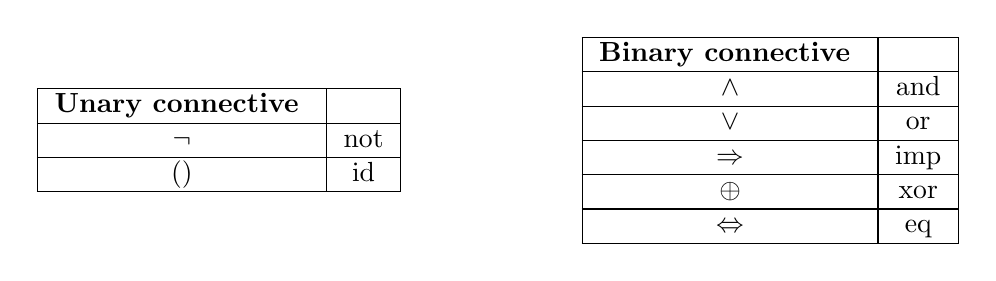
\begin{tikzpicture}
\node [anchor=center] at (0,0) {
	\begin{tabular}{|c|c|}
  	\hline
 	\textbf{Unary connective $\exconnective$} & \textbf{$\synencodingof{\exconnective}$} \\
  	\hline
 	$\lnot$ 	&  \stringof{not} \\
  	\hline
 	$()$		&  \stringof{id} \\
  	\hline
	\end{tabular}};
\node [anchor=center] at (7,0) {
	\begin{tabular}{|c|c|}
  	\hline
 	\textbf{Binary connective $\exconnective$} & \textbf{$\synencodingof{\exconnective}$} \\
  	\hline
 	$\land$ 		&  \stringof{and} \\
  	\hline
 	$\lor$ 		&  \stringof{or} \\
  	\hline
 	$\Rightarrow$ 	&  \stringof{imp} \\
  	\hline
	 $\oplus$ 		&  \stringof{xor} \\
  	\hline
	 $\Leftrightarrow$ &  \stringof{eq} \\
  	\hline
	\end{tabular}};
\end{tikzpicture}
\end{center}

% WOLFRAM Numbers
Besides these specific connectives we exploit a generic representation scheme of propositional formulas by the so-called Wolfram code orginially designed for the classification of cellular automaton rules \cite{wolfram_statistical_1983} and popularized in the book \cite{wolfram_new_2002}.
Along this, the coordinate encodings of connectives $\exconnective$ with differing arity are flattened and interpreted as a binary number, which is transformed into a decimal number and represented as a string $\synencodingof{\exconnective}$.
We then choose a prefix to encode the arity by
\begin{itemize}
	\item \stringof{u} for unary
	\item \stringof{b} for binary
	\item \stringof{t} for ternary
	\item \stringof{q} for quarternary
\end{itemize}
connectives.
Together, the connective is represented by the string concatenation
	\[  \synencodingof{\exconnective} = \synencodingof{\catorder} + \synencodingof{\exconnective} \, . \]


% Atoms
\textbf{Atomic Formulas} are represented by arbitrary strings, which are not used for the representation of connectives.
We further avoid the symbols \{\stringof{(}, \stringof{)}, \stringof{\_}\} in the names of atoms, to not confuse them with colors of categorical variables.

% Composed Formulas
\textbf{Composed Formulas} $\exformula_1\exconnective,\exformula_2$ are represented by
\begin{centeredcode}
	$\synencodingof{\exformula_1\exconnective,\exformula_2}$ = [$\synencodingof{\exconnective}$, $\synencodingof{\exformula_1}$, $\synencodingof{\exformula_2}$]
\end{centeredcode}
where we apply the conventions
\begin{itemize}
	\item Connectives are at the 0th position in each list
	\item Further entries are either atoms as strings or encoded formulas itself
\end{itemize}

% Backus-Naur
The applied grammar in Backus-Naur form is \\
\begin{tabular}{|l|l|}
  	\hline
 	Unary Connective & \stringof{not} | \stringof{id}\\
  	\hline
 	Binary Connective & \stringof{and} | \stringof{or} | \stringof{imp} | \stringof{xor}  | \stringof{eq} \\
  	\hline
 	Atomic Formula & Set of strings not in Connectives\\
  	\hline
	Complex Formula & Atomic Formula | [Unary Connective, Complex Formula] | \\
	&  [Binary Connective, Complex Formula, Complex Formula] \\
	\hline
\end{tabular}


\begin{example}[Encoding of the Wet Street example]
For example we have
\begin{itemize}
	\item
	Atomic variable $\var{Rained}$ by
		\begin{centeredcode}
			$\synencodingof{\var{Rained}}$
			= \stringof{Rained}
		\end{centeredcode}
	\item
	Negative literal $\lnot\var{Rained}$ by
		\begin{centeredcode}
			$\synencodingof{\lnot\var{Rained}}$
			= [\stringof{not},\stringof{Rained}]
		\end{centeredcode}
	\item
	Horn clause $\left(\var{Rained}\Rightarrow\var{Wet}\right)$ by
		\begin{centeredcode}
			$\synencodingof{\var{Rained}\Rightarrow\var{Wet}}$
			= [\stringof{imp},\stringof{Rained},\stringof{Wet}]
		\end{centeredcode}
	\item
	Knowledge Base
	$(\lnot\var{Rained})\land(\var{Rained}\Rightarrow\var{Wet})$ by
		\begin{centeredcode}
			$\synencodingof{\lnot\var{Rained})\land(\var{Rained}\Rightarrow\var{Wet}}$
			=  [\stringof{and}, [\stringof{not}, \stringof{Rained}], [\stringof{imp}, \stringof{Rained}, \stringof{Wet}]]
		\end{centeredcode}
\end{itemize}
\end{example}




\textbf{Knowledge Bases}

% Should distinguish these in knowledge?
We distinguish here formulas, with propositional logic interpretation and formulas which have a soft logic interpretation.
%\textbf{Facts.}
The formulas with hard interpretation are called facts in a knowledge base $\kb$ and encoded by dictionaries
\begin{centeredcode}
	\{key($\exformula$) : $\synencodingof{\exformula}$ for $\exformula\in\kb$ \}
\end{centeredcode}

\textbf{Markov Logic Networks}

%\textbf{Weighted formulas.}
The formulas with soft interpretation are called weighted formulas and encoded by $\expof{\weightof{\exformula}\cdot\exformula}$.
We thus require a specification of the weights, which we do by adding $\weightof{\exformula}$ as a $\mathrm{float}$ or an $\mathrm{int}$ to the list $\synencodingof{\exformula}$.
We then store Markov Logic Networks by dictionaries
\begin{centeredcode}
	\{key($\exformula$) : $\synencodingof{\exformula}$ + [$\weightof{\exformula}$] for $\exformula\in\formulaset$\}
\end{centeredcode}

\textbf{Neuro-Symbolic Architecture by Nested Lists}

% Generalizing the script language to specify architectures
To specify neuro-symbolic architectures in terms of formula selecting maps, as has been the subject of \charef{cha:formulaSelection} we further exploit the nested list structure of encoding propositional logics.
We replace, in each hierarchy of the nested structure each entry by a list of possible choices.
In this way, we reinterpret the list index as the choice indices $\selindex$ introduced for connective and formula selections (see \defref{def:connectiveSelector} and \ref{def:formulaSelector}).

% Neurons
A connective selector (see \defref{def:connectiveSelector}) is encoded by the list
	\begin{centeredcode}
			$\synencodingof{\exconnective}$
			= [$\synencodingof{\exconnective_{0}}$, $\ldots$, $\synencodingof{\exconnective_{\seldim\shortminus1}}$]
	\end{centeredcode}
and a formula selector (see \defref{def:formulaSelector}) by
	\begin{centeredcode}
			$\synencodingof{\fselectionmap}$
			= [$\synencodingof{\exconnective_{0}}$, $\ldots$, $\synencodingof{\exconnective_{\seldim\shortminus1}}$]
	\end{centeredcode}
A logical neuron of order $\selorder$ (see \defref{def:fsNeuron}), defined by a connective selector $\exconnective$, and a formula selector $\fselectionmap_\atomenumerator$ on each argument $\atomenumerator\in[\selorder]$, is encoded by
		\begin{centeredcode}
			$\synencodingof{\lneuron}$
			= [$\synencodingof{\exconnective}$, $\synencodingof{\fselectionmap_0}$, $\ldots$,  $\synencodingof{\fselectionmap_{\selorder-1}}$]
		\end{centeredcode}
Only the unary $\selorder=1$ and the $\selorder=2$ cases are supported.


% Confusing?
The resulting nested lists indices have an alternating interpretation at each level compared with the elements of each list.
That is, when $\synencodingof{\lneuron}$ is the encoding of a neuron, then any element $x\in\synencodingof{\lneuron}$ represents a list of choices.
When $x$ is not the first element, then each choice is either the encoding $\synencodingof{\catvariable}$ of an atomic formula, or another neuron.

% Find another symbol?
A neural architecture $\larchitecture$ is then represented in the dictionary
\begin{centeredcode}
	$\synencodingof{\larchitecture}$ = \{key($\lneuron$) : $\synencodingof{\lneuron}$ for $\exformula\in\larchitecture$\}
\end{centeredcode}
%To store this structure, we choose dictionaries of neuron spe
%\begin{centeredcode}
%	\{key($\lneuron$) : $\synencodingof{\lneuron}$ for $\exformula\in\formulaset$\}
%\end{centeredcode}
where key($\lneuron$) is a string, which can be used in the formula selections of other neurons.

% Important for well-definedness
It is important that the directed graph of neurons induced by the choice possibilities is acyclic, to ensure well-definedness of the architecture.


% Backus-Naur
In order to represent neuro-symbolic architectures, the grammar of $\synencodingof{\cdot}$ in Backus-Naur Form is extended by the production rules \\
\begin{tabular}{|l|l|}
  	\hline
 	Unary Connectives & [Unary Connective] | [Unary Connective] + Unary Connectives \\
  	\hline
 	Binary Connectives & [Unary Connective] | [Binary Connective] + Binary Connectives \\
	%\hline
	%Neuron Name & Any set of strings not used for atoms or connectives \\
  	\hline
 	Dependency Choice & Atomic Formula | Neuron \\
  	\hline
	Dependency Choices & [Dependency Choice] | [Dependency Choice] + Dependency Choices \\
	\hline
	Neuron & [Unary Connectives, Dependency Choices] | \\
	&  [Binary Connectives, Dependency Choices, Dependency Choices] \\
	\hline
\end{tabular}


\begin{example}[Neuro-Symbolic Architecture for the Wet Street]
	Following the wet street example, we can define a neuron by
	\begin{centeredcode}
		$\synencodingof{\lneuron}$ = [[\stringof{imp},\stringof{eq}],[\stringof{Wet},\stringof{Sprinkler}],[\stringof{Street}]]
	\end{centeredcode}
	from which the formulas
	\begin{centeredcode}
		[\stringof{imp}, \stringof{Wet}, \stringof{Street}] \\
		\hspace{0.25cm} [\stringof{eq}, \stringof{Wet}, \stringof{Street}] \\
		\hspace{1cm}[\stringof{imp}, \stringof{Sprinkler}, \stringof{Street}] \\
		\hspace{1cm}[\stringof{eq}, \stringof{Sprinkler}, \stringof{Street}]
	\end{centeredcode}
	can be chosen.
	Combining this neuron with further neurons, e.g. by the architecture
	\begin{centeredcode}
		$\synencodingof{\larchitecture}$ = \{ \stringof{neur1}: [[\stringof{imp},\stringof{eq}],[\stringof{neur2}],[\stringof{Street}]] , \\
		\hspace{1.8cm}\stringof{neur2}: [[\stringof{lnot},\stringof{id}],[\stringof{Wet},\stringof{Sprinkler}],[\stringof{Street}]] \}
	\end{centeredcode}
	the expressitivity increases.
	In this case, the further neuron provides the flexibility of the first atoms to be replaced by its negation.
\end{example}



\subsect{Distributions}

We encode Markov Networks by specifying a set of tensor cores.
Each distribution needs to have a routine
\begin{lstlisting}
	.create_cores()
\end{lstlisting}
creating the factor cores and 
\begin{lstlisting}
	.get_partition_function()
\end{lstlisting}
calculating the partition function.
Although the partition function can be calculated by the contraction of all cores, we separate the method since there are situations where a faster calculation can be performed.


\textbf{Empirical Distributions} are distributions of sample data.
We represent the values as a CP Format of data cores as specified in \secref{sec:empDistribution}
\begin{lstlisting}
	knowledge.EmpiricalDistribution
\end{lstlisting}
Here the partition function is the number of samples used in the creation of the empirical distribution.


\textbf{HybridKnowledgeBases} are probability distributions, which are specified by propositional formulas in the script language.
\begin{lstlisting}
	knowledge.HybridKnowledgeBase
\end{lstlisting}
They are initialized with arguments
\begin{itemize}
	\item facts: Dictionary of propositional formulas stored as $\synencodingof{\exformula}$ representing hard logical constraints
	\item weightedFormulas: Dictionary of propositional formulas stored as $\synencodingof{\exformula}$+$[\weightof{\exformula}]$ representing soft logical constraints
	\item evidence: Dictionary of atomic formulas, where key are the formulas in string representation and values the certainty in $[0,1]$ (float or int) of the atom being true
	\item categoricalConstraints: Dictionary of categorical constrained, which values are lists of atomic formulas stored as strings $\synencodingof{\atomicformula}$
\end{itemize}


\subsect{Inference}

By
\begin{lstlisting}
	knowledge.InferenceProvider
\end{lstlisting}
taking a distribution from the above as argument.

% Probabilistic Queries
Probabilistic queries as specified \defref{def:queries})  by
\begin{lstlisting}
	.query(variableList, evidenceDict)
\end{lstlisting}

MAP queries by
\begin{lstlisting}
	.exact_map_query()
\end{lstlisting}
or by
\begin{lstlisting}
	.annealed_sample()
\end{lstlisting}
using Simulated Annealing (see Remark~\ref{rem:simulatedAnnealing}) to find an approximate maximum.
The second method circumvents the creation of the coordinatewise representation of the distribution and circumvents therefore, at the expense of potentially approximative solutions, a bottleneck in case of many query variables.

% Entailment Queries
Entailment from the distribution (\defref{def:entailment}) is be decided by
\begin{lstlisting}
	.ask(queryFormula, evidenceDict)
\end{lstlisting}
where queryFormula is the formula $\exformula$ to be tested for entailment in the representation $\synencodingof{\exformula}$.

% Sampling
Samples can be drawn by
\begin{lstlisting}
	.draw_samples(sampleNum, variableList, annealingPattern)
\end{lstlisting}
based on Gibbs sampling, where
\begin{itemize}
	\item sampleNum (int) gives the number of samples to be drawn
	\item variableList (list of str) defines the variables to be represented by the samples (default: all atoms in the distribution)
	\item annealingPattern specifies an annealing pattern 
\end{itemize}


\subsect{Parameter Estimation}

\textbf{EntropyMaximizer} implements Algorithm~\ref{alg:AWO}, which is motivated by the maximum entropy principle (see \secref{sec:maxEntDuality}) to optimize Markov Logic Networks.
The class  
\begin{lstlisting}
	knowledge.EntropyMaximizer
\end{lstlisting}
is initialized with the arguments
\begin{itemize}
	\item expressionsDict: Dictionary of formulas in the format $\synencodingof{\exformula}$ 
	\item satisfactionDict: Dictionary of the satisfaction rates (mean parameters) to be matched by the optimal distribution
\end{itemize}
The optimization is then performed by
\begin{lstlisting}
	.alternating_optimization(sweepNum, updateKeys)
\end{lstlisting}
method, where the iteration in Algorithm~\ref{alg:AWO} through the updateKeys is performed sweepNum times.

\subsect{Structure Learning}

\textbf{Formula Booster} chooses a formula given a formula selecting map.
\begin{lstlisting}
	knowledge.FormulaBooster
\end{lstlisting}
is initialized with the arguments
\begin{itemize}
	\item knowledgeBase: Distribution representing a current model to be improved
	\item specDict: A neuro-symbolic architecture encoded in a dictionary of neurons
\end{itemize}


